\subsubsection{Rancangan Detail Komponen Logging}
\label{subsubsection:detail-data-logging}

Komponen \textit{logging} dan \textit{tracing} bertanggung jawab untuk mencatat dan melacak aktivitas sistem. Komponen ini akan mengumpulkan data dari berbagai komponen lain dalam sistem, termasuk informasi tentang permintaan yang diterima, respons yang dikirim, dan status sistem secara keseluruhan. Data ini akan digunakan untuk analisis lebih lanjut dan pemecahan masalah.

Ilustrasi struktur komponen \textit{logging} dan \textit{tracing} dapat dilihat pada gambar \ref{fig:logging-tracing-structure}.

% _TODO: Change image
\begin{figure}[ht]
    \centering
    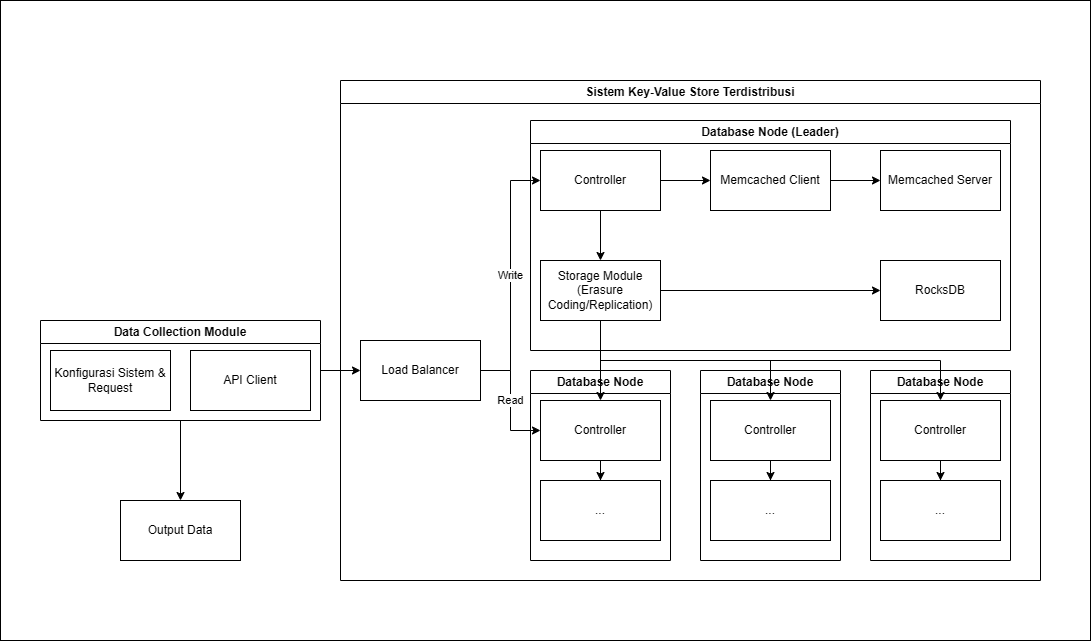
\includegraphics[width=0.95\textwidth]{resources/chapter-3/general-architecture.png}
    \caption{Struktur Komponen Logging dan Tracing}
    \label{fig:logging-tracing-structure}
\end{figure}